\subsubsubsubsection{Street}
\begin{figure}[h]
\centering
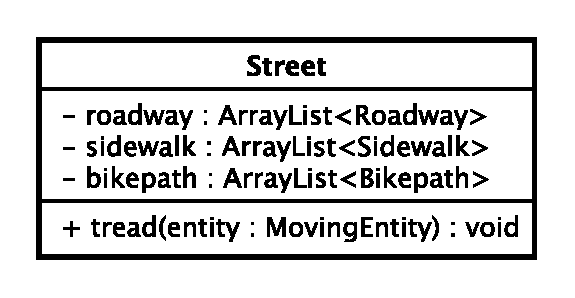
\includegraphics[scale=0.6,keepaspectratio]{images/solution/street.eps}
\caption{App::Reactive::Street}
\label{fig:sd-app-street}
\end{figure}
\FloatBarrier
\begin{itemize}
  \item \textbf{Description} \\
    It represents a concrete street.
  \item \textbf{Attribute}
  \begin{itemize}
    \item \texttt{- roadway: ArrayList<Roadway>} \\
A street is composed by roadways.
    \item \texttt{- sidewalk: ArrayList<Sidewalk>} \\
A street is composed by sidewalks, typically one for each side
of the street.
    \item \texttt{- bikepath: ArrayList<Bikepath>} \\
A street is composed by bikepaths, typically one for each side
of the street.
  \end{itemize}
  \item \textbf{Operation}
  \begin{itemize} 
    \item \texttt{+ tread(entity: MovingEntity)} \\
Moves the entity in the correct part of the street based on the 
concrete type of the entity (i.e. a pedestrian will tread a sidewalk).
  \end{itemize}
\end{itemize}
